% Ellis Masters Project Report % 
% Required Packages %
\documentclass[12 pt]{report}
\usepackage[margin=1 in]{geometry}
\usepackage{amsmath}
\usepackage{graphicx}
\usepackage{xspace}
\usepackage[style=ieee, url=false]{biblatex}
\usepackage{parskip} % adds a skipped paragraph
\addbibresource{bibliography/jetpump.bib}

\newcommand{\Mach}{\mbox{\textit{Ma}}}  % Mach number
\newcommand{\dete}{$\mathrm{dE_{te}}$\xspace}  % Throat Entry Equation
\newcommand{\dedi}{$\mathrm{dE_{di}}$\xspace}  % Throat Entry Equation
\newcommand{\pte}{$\mathrm{P_{te}}$\xspace}  % Pressure Throat Entry Equation
\newcommand{\pnz}{$\mathrm{P_{nz}}$\xspace}  % Pressure Nozzle Tip
\newcommand{\pni}{$\mathrm{P_{ni}}$\xspace}  % Pressure Nozzle Tip
\newcommand{\pdi}{$\mathrm{P_{di}}$\xspace}  % Pressure Nozzle Tip
\newcommand{\pdiA}{$\mathrm{P_{di}^{A}}$\xspace}  % Pressure Discharge Available
\newcommand{\pdiR}{$\mathrm{P_{di}^{R}}$\xspace}  % Pressure Discharge Required

\title{Jet Pump Model for Oil Wells}
\author{Kaelin Ellis}
\date{September 2024}

\begin{document}

\maketitle

\section{Technical Introduction}

Jet pumps are simple devices with no moving parts. They take advantage of the fluid energy relationship to transfer pressure energy into kinetic energy, combine two fluid’s kinetic energies and then re-convert the kinetic into pressure again. With that being said, some complexities of jet pumps exist, especially when operating in multiphase flow as an oil jet pump does. The complexities arise when trying to model the behavior of the reservoir fluid while it flows into the jet pump. As the reservoir fluid speeds up, kinetic energy is increased, which creates a drop in pressure, liberating gas from the solution. The multiphase phase mixture of oil, water and gas has a sonic velocity that is much lower than the individual components of pure liquid or pure vapor.  The combination of a high mixture velocity and a low sonic velocity creates an inconvenient situation, where the fluid can hit its sonic flow limitation. Once the sonic velocity is reached, no further reduction in discharge pressure has an effect on the flow through the pump. A dynamic boundary is reached, with the only solution being a new jet pump with a larger flow area. Properly calculating the sonic velocity of a multiphase mixture is critical to capturing the behavior of a multiphase jet pump.

\section{Sonic Velocity}

Sonic velocity is the speed that sound moves through a fluid. The sound propagates as a wave, where one particle comes into contact with another. These interactions cascade which allows sound to be transmitted from one location to another. The same phenomenon occurs when a fluid flows through a pipe. The particles move forward with a bulk velocity, but internally in the pipe, fluid interactions are also occurring. The reason the fluid flows along the pipe at the same mass flow rate is because the bulk velocity is operating below the sonic velocity. Said in another manner, the bulk speed of the fluid is less than how quickly the particles can move away from each other. Attempting to flow faster than the sonic velocity creates an accumulation of particles which in turn slows down the fluid to below its sonic velocity. Specialized devices exist that can eliminate the accumulation and accelerate the fluid above its sonic velocity, but they are not pertinent to this report. The next section will explore computing the properties required for predicting a multiphase mixture sonic velocity.

The properties required for predicting sonic velocity are the modulus of elasticity, K and the fluid density, $\rho$. The modulus of elasticity is how much deformation a fluid will experience under pressure. In the analysis a homogeneous mixture is assumed for the fluid as it flows into the jet pump. Calculating the mixtures modulus of elasticity and density are displayed in equations \eqref{mix_elas} and \eqref{mix_dens} respectively. As seen, the mixture modulus of elasticity is dependent on the volume fractions of the oil, water and gas. The mixture density is dependent on the mass fractions of the components.

\begin{equation}
\frac{1}{K_{mix}} = \frac{y_{o}}{K_{o}} + \frac{y_{w}}{K_{w}} + \frac{y_{g}}{K_{g}}
\label{mix_elas}
\end{equation}

\begin{equation}
\frac{1}{\rho_{mix}} = \frac{m_{o}}{\rho_{o}} + \frac{m_{w}}{\rho_{w}} + \frac{m_{g}}{\rho_{g}}
\label{mix_dens}
\end{equation}

With the appropriate mixture properties, the standard equation for calculating the sonic velocity of a fluid is used, displayed in equation \eqref{speed_sound}. 

\begin{equation}
c_{mix} = \sqrt{\frac{K_{mix}}{\rho_{mix}}}
\label{speed_sound}
\end{equation}

The Mach number is a dimensionless number that compares the velocity a fluid is flowing to its speed of sound, represented in equation \eqref{mach_no}.

\begin{equation}
Ma = \frac{v_{mix}}{c_{mix}}
\label{mach_no}
\end{equation}

Any Mach number of 1.0 or greater is sonic. Flow can also be described sonically by the categories listed below.

\begin{itemize}
    \item Subsonic: $Ma \leq 0.8$
    \item Transonic: $0.8 < Ma < 1.2$
    \item Supersonic: $1.2 \leq Ma$
\end{itemize}

The boundary limit for oil well jet pumps is a Mach value of 1 or below.

As previously said, a multiphase mixture of vapor and liquid has the inconvenient property of its mixture velocity being less than the individual components \cite{himr}. An example of this is a mixture of air and water. The individual components of air and water have a sonic velocity of 1100 and 5000 ft/s respectively. Combining these fluids in a 50/50 mixture results in a sonic velocity of 300 ft/s, nearly a quarter less than the sonic velocity of the air by itself. The relationship of sonic velocity and mixture velocity will be explored more in the detailed discussions on the jet pump throat entrance. Before progressing to the throat entrance, further background is needed on the fundamental equations for a jet pump, namely the fluid energy equation.

\section{Fluid Energy Equation}

The one dimensional fluid energy equation \eqref{raw_energy} provides the foundation for compressible flow in conduits \cite{fluids_cheme}. The energy equation states that the differences in potential energy, pressure energy, kinetic energy, friction and work have to be equal.

\begin{equation}
gdz + \frac{dP}{\rho} + vdv + dF = dW
\label{raw_energy}
\end{equation}

For a jet pump, the potential energy and work terms can be omitted. The equation simplifies to the jet pump energy equation \eqref{jpump_energy}.

\begin{equation}
\frac{dP}{\rho} + vdv + dF = 0
\label{jpump_energy}
\end{equation}

Fluid flow across a jet pump nozzle tip, throat entrance and diffuser can all be modeled using variations of the jet pump energy equation. The details on these different components will be detailed in the next sections.

\begin{figure}
    \centering
    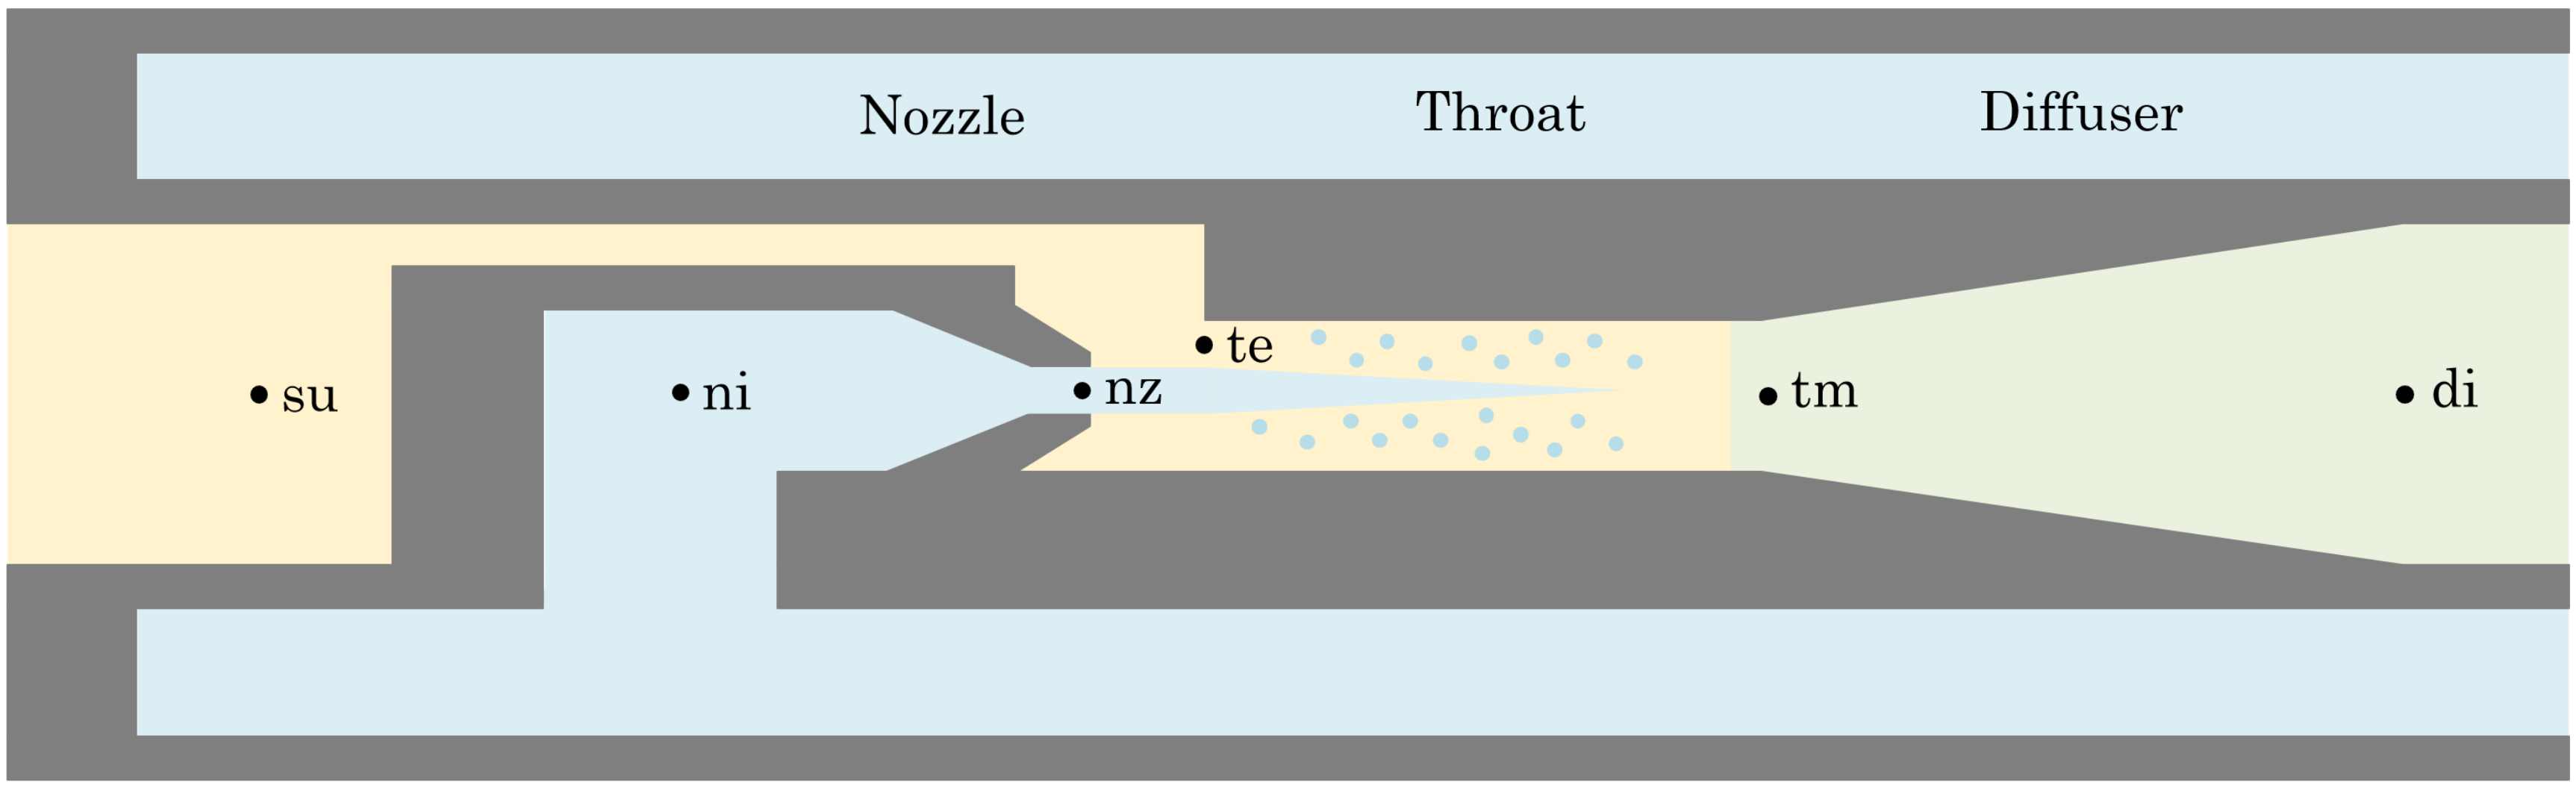
\includegraphics[width=1\linewidth]{figures/jp_over_v2.PNG}
    \caption{Jet Pump Overview}
    \label{fig:jetpump_side}
\end{figure}

\section{Jet Pump Components}

A jet pump is a made up of three mechanical components which are the nozzle, throat and diffuser. Six reference locations are assigned inside the jet pump for differences in pressure or fluid properties. The reference locations are the suction (su), nozzle inlet (ni), nozzle tip (nz), throat entrance (te), throat mixture (tm) and diffuser outlet (di). Figure \ref{fig:jetpump_side} provides a sketch of the geometry of a jet pump. 

\section{Nozzle Size and Throat Ratio}

A jet pump is identified by a nozzle number and a throat ratio. The nozzle number is an integer with a value of 1 to 20, each corresponding to a specific diameter. The throat ratio is a letter of the form X, A, B, C, D or E which is the throat diameter divided by the nozzle diameter. An example of the identification is 11X, 13C, or 9D. Table \ref{tab:national_jp_ratios} shows the numeric ratios at each letter.

\begin{table}[h]
\centering
\begin{tabular}{|c|c|c|c|c|}
\hline
Ratio & Nozzle & Throat & Area Ratio & Dia. Ratio \\
\hline
X & N & N - 1 & 2.07 & 1.44 \\
A & N & N & 2.63 & 1.62 \\
B & N & N + 1 & 3.34 & 1.83 \\
C & N & N + 2 & 4.26 & 2.06 \\
D & N & N + 3 & 5.43 & 2.33 \\
E & N & N + 4 & 6.90 & 2.63 \\
\hline
\end{tabular}
\caption{Jet Pump Throat to Nozzle Ratios}
\label{tab:national_jp_ratios}
\end{table}

Specifying jet pumps in this manner allows quick generalities to be made about the behavior. An X pump will provide the largest head, but the smallest suction flow for a given nozzle. Likewise an E will provide the smallest head, but the largest suction flow for a given nozzle.

Instead of using the specified ratios to calculate the throat diameter a lookup table can be used. Table \ref{tab:national_jp_dims} are the jet pump dimensions offered by National Jet Pumps \cite{world_oil_one}. As shown both the nozzle and throat have a unique number that identifies the diameter. Columns 2 and 3 in table \ref{tab:national_jp_ratios} show how those numbers can be used to find the exact diameter of the nozzle and throat. A list of examples are provided.

\begin{itemize}
    \item 11X Jet Pump - 11 Nozzle with 10 Throat
    \item 12C Jet Pump - 12 Nozzle with 14 Throat
    \item 13A Jet Pump - 13 Nozzle with 13 Throat
\end{itemize}

\begin{table}[h]
\centering
\begin{tabular}{|c|c|c|c|}
\hline
Nozzle & Nozzle & Throat & Throat \\
No. & Dia. & No. & Dia. \\
 & inches &  & inches \\
\hline
1 & 0.0553 & 1 & 0.0903 \\
2 & 0.0628 & 2 & 0.1016 \\
3 & 0.0705 & 3 & 0.1151 \\
4 & 0.0798 & 4 & 0.1291 \\
5 & 0.0903 & 5 & 0.1458 \\
6 & 0.1016 & 6 & 0.1643 \\
7 & 0.1145 & 7 & 0.1858 \\
8 & 0.1291 & 8 & 0.2099 \\
9 & 0.1458 & 9 & 0.2370 \\
10 & 0.1643 & 10 & 0.2675 \\
11 & 0.1858 & 11 & 0.3017 \\
12 & 0.2099 & 12 & 0.3404 \\
13 & 0.2370 & 13 & 0.3841 \\
14 & 0.2675 & 14 & 0.4335 \\
15 & 0.3017 & 15 & 0.4981 \\
16 & 0.3404 & 16 & 0.5519 \\
17 & 0.3841 & 17 & 0.6228 \\
18 & 0.4335 & 18 & 0.7027 \\
19 & 0.4981 & 19 & 0.7929 \\
20 & 0.5519 & 20 & 0.8947 \\
\hline
\end{tabular}
\caption{National Nozzle and Throat Sizes}
\label{tab:national_jp_dims}
\end{table}

\section{Throat Entrance}

The throat entrance contains the most complex fluid dynamics of all the jet pump sections. The pressure obtained at the throat entrance cascades across to the nozzle, throat and diffuser. As such it is the natural starting point.

The reservoir fluid starts its flow into the suction of the jet pump and is then constricted down through the throat entrance. The area of the throat entrance is equal to the throat area minus the nozzle jet area. At the throat entrance, the power fluid from the nozzle is in a continuous jet taking away valuable space for the reservoir fluid to flow. Figure \ref{fig:jetpump_side} shows how the jet is occupying space at the throat entrance.

To properly model the fluid in the throat entrance, an accurate description needs to be obtained. The reservoir fluid is a three phase mixture, which does not behave as an ideal gas and the liquid is continually liberating gas into the vapor phase. As such, minimal assumptions can be applied to the fluid energy equation to simplify it. The only assumption that can be applied is that the velocity of the reservoir fluid at the pump suction is negligible compared to the velocity at the throat entrance. The energy equation \eqref{jpump_energy} is rewritten specifically for the throat entrance as equation \eqref{entr_intg}.

\begin{equation}
% The vphantom gets the vertical alignment of the underbraces
dE_{te} = \int_{su}^{te} \frac{dP}{\rho} + \frac{v_{te}^{2}}{2} * (1+K_{en}) = 0
\label{entr_intg}
\end{equation}

The term \dete stands for differential energy of the throat entrance. The equation calculates the difference in energy between the fluid at the suction and at the throat entrance. To have physical meaning, the \dete term needs to equal zero.

As previously stated, equation \eqref{entr_intg} is the farthest the energy equation can analytically be simplified. Analytically integrating an equation that describes the density of a three phase mixture with a gas soluble liquid and a non-ideal gas would be formidable. To simplify the problem, the analytical integration is turned into a numerical integration using the trapezoidal rule. Equation \eqref{entr_trap} shows the numerical solution of the throat entrance energy equation.

\begin{equation}
% The vphantom gets the vertical alignment of the underbraces
dE_{te} = \underbrace{\frac{\Delta P}{2}\sum_{k=su}^{te} (\frac{1}{\rho_{k}} + \frac{1}{\rho_{k+1}})}_{\text{Expansion Energy}} + \underbrace{\vphantom{\sum_{k=su}^{te}}{\frac{v_{te}^{2}}{2} * (1+K_{en})}}_{\text{Kinetic Energy}} = 0
\label{entr_trap}
\end{equation}

For ease of discussion \dete is split into two terms. The first term is the expansion energy, which represents the energy change from pressure differences. The second term is the kinetic energy, which accounts for energy related to the fluid's velocity and friction. The solution value of \pte{} is obtained when the kinetic and expansion energy sum to zero. This is achieved with iteration, with the detailed steps outlined below.
\begin{enumerate}
    \item Select a small pressure delta to step the suction pressure down
    \item Reduce pressure by the delta 
    \item Calculate the reservoir fluid specific volume, throat entrance velocity, and sonic velocity 
    \item Integrate the area under the specific volume curve for the expansion energy
    \item Square the throat entrance velocity for the kinetic energy
    \item Add the kinetic energy and expansion energy together for \dete{}
    \item Four variations in outcome can occur:
    \begin{enumerate}
        \item \dete{} is positive and the Mach number is below one. Continue reducing the pressure by the delta step.
        \item \dete{} is positive and the Mach number is greater than or equal to one. The suction flow rate selected was too high for the suction pressure. Select a new suction flow rate and pressure.
        \item \dete{} is negative and the Mach number is below one. A non-choked solution was found for \pte.
        \item \dete{} is negative and the Mach number is greater than or equal to one. A choked solution was found for \pte.
    \end{enumerate}
\end{enumerate}

Figure \ref{fig:dete_multi} is a plot of the \dete{} for five difference suction pressures and different flow rates. The legend has values for suction pressure and flow rate, which are set by the reservoir conditions. Only the barrels of oil produced are displayed instead of also including the natural gas and water.

\begin{figure}
    \centering
    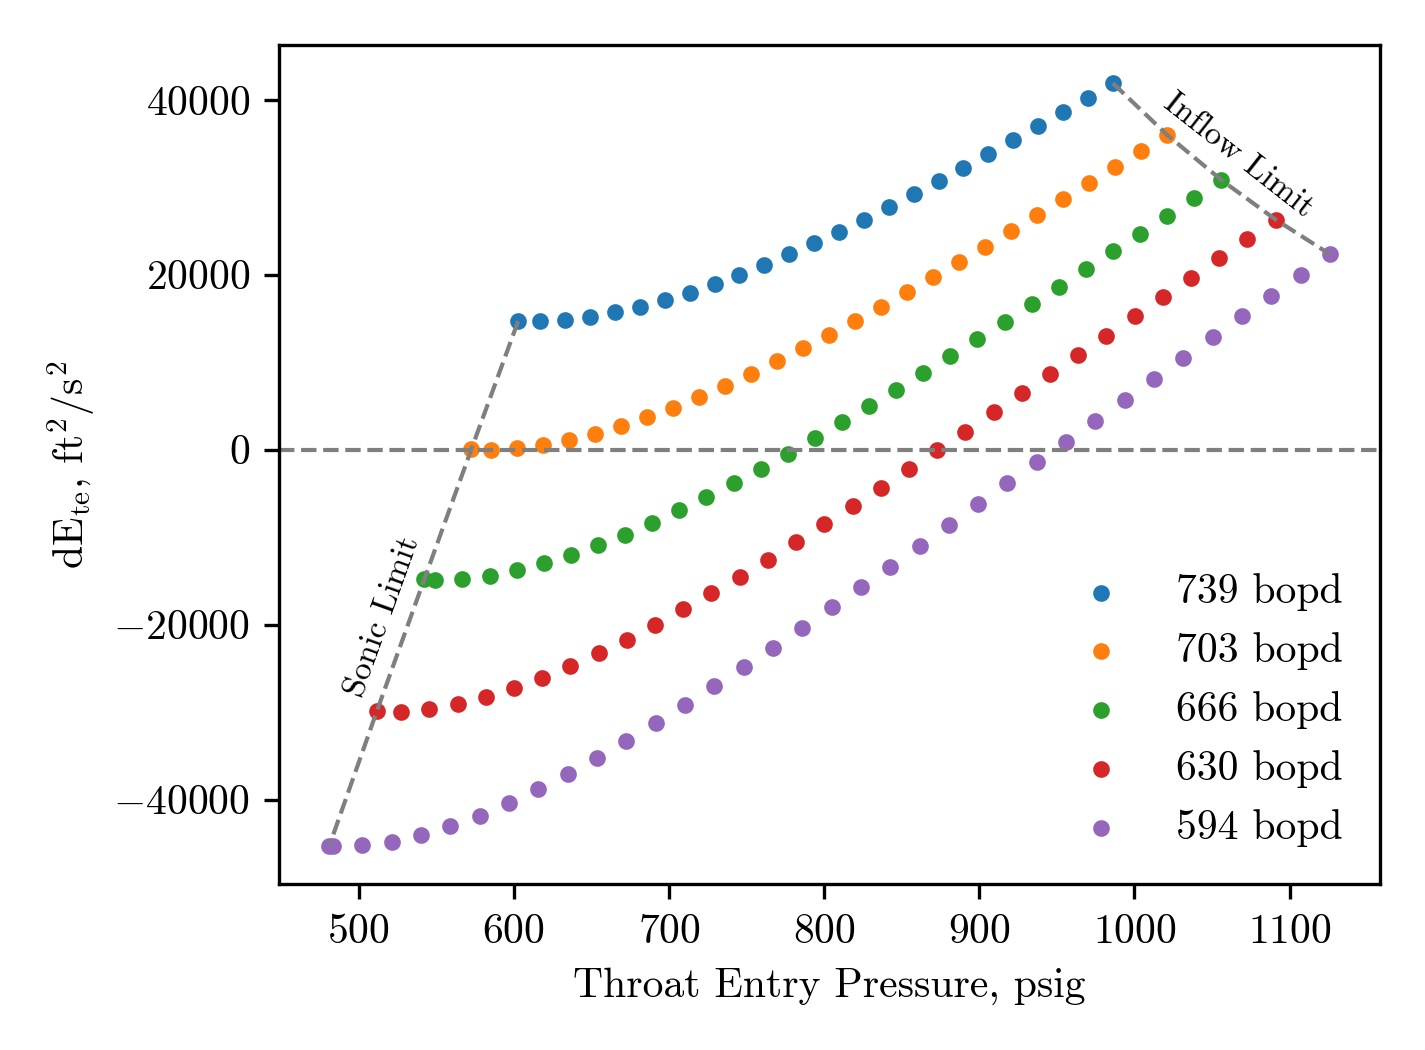
\includegraphics[scale=1]{figures/entry_multi.png}
    \caption{\dete at Different Suction Conditions}
    \label{fig:dete_multi}
\end{figure}

Figure \ref{fig:dete_multi} has two boundary lines, the inflow limit and the sonic limit. The inflow limit is determined by the reservoir fluid productivity at different suction pressures. The sonic limit is where the fluid is traveling at Mach one inside the throat entrance. These boundary's provide tangible starting and stopping points for iteration. Solutions for \pte{} are seen where the line crosses the \dete{} zero axis. The highest flow rate shows a suction pressure that was chosen to be too low. The line starts at the inflow limit, but does not have enough pressure to convert to the required kinetic energy. As a result, the sonic limit is contacted before crossing the zero axis with \dete{}. A new suction pressure with a higher pressure needs to be used.

Further detail on the variables that go into \dete{} are shown in figure \ref{fig:entr_four} for a singular suction pressure and flow rate. This graph provides details on the specific volume, mixture velocity, sonic velocity and separate expansion and kinetic energies. Also, the graph of \dete is not truncated above a Mach number of one. Looking more closely at the \dete graph one can observe the slope of the curve transitioning from a positive to a negative slope. The transition of the slope occurs as the jet pump is operating in transonic flow. Where the slope of the line is zero coincides with a Mach value of one. A full derivation from first principle equations is provided in Appendix A. The end result of the derivation is equation \eqref{dete_dp}.

\begin{figure}
    \centering
    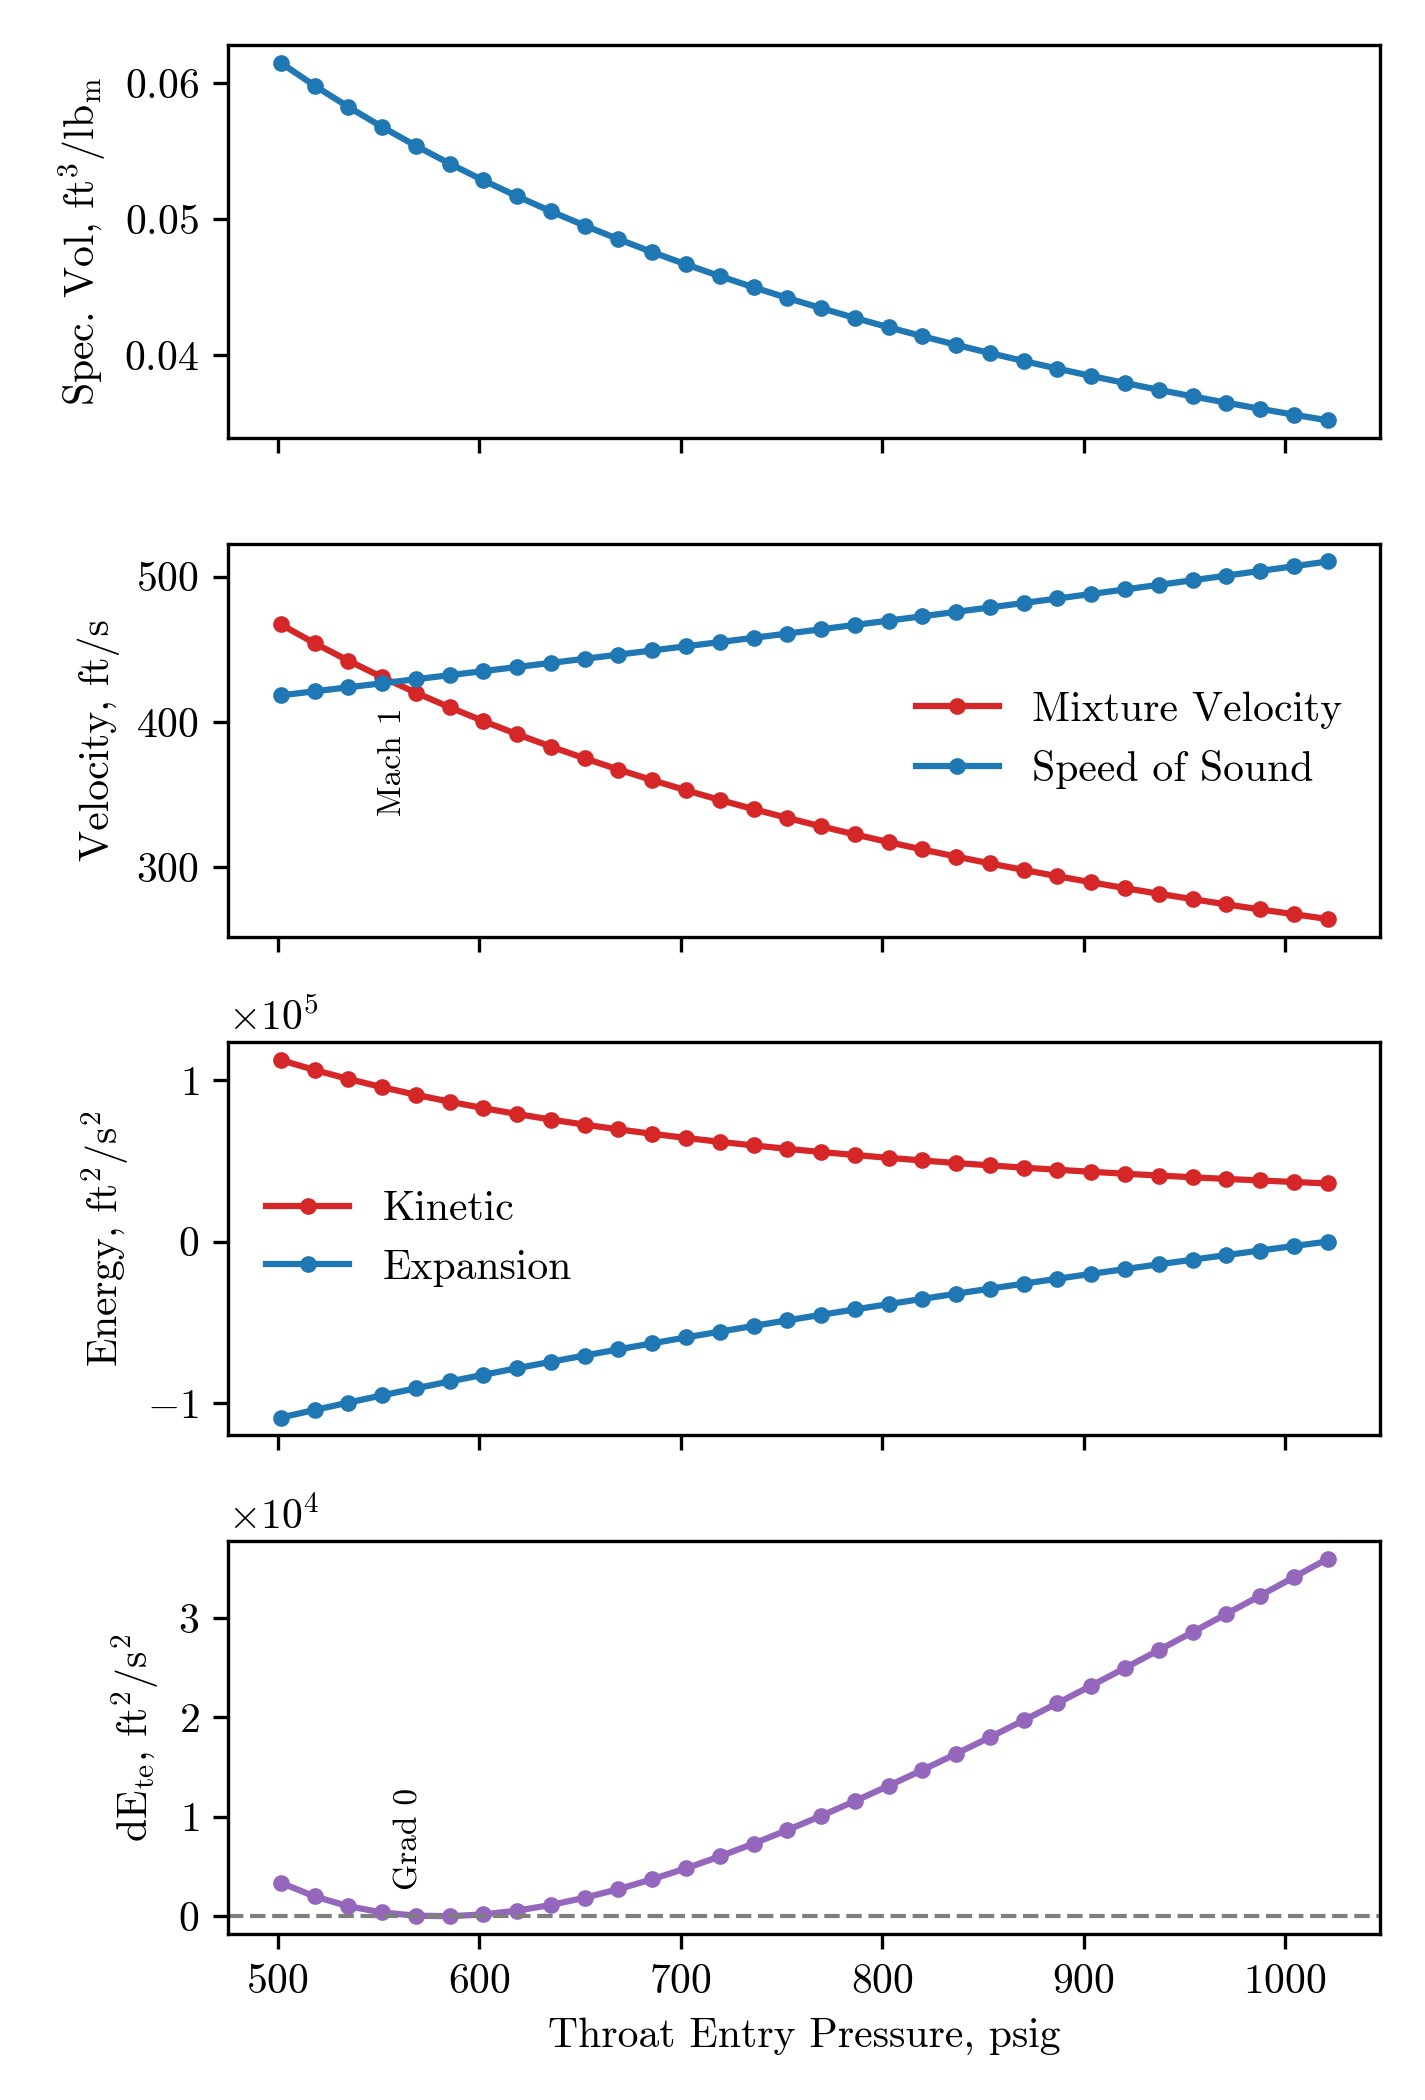
\includegraphics[scale=1]{figures/entry_four.png}
    \caption{Properties for Calculating Throat Entry Pressure}
    \label{fig:entr_four}
\end{figure}

\begin{equation}
\frac{dE_{te}}{dP} = \frac{1}{\rho}(1 - \Mach^2)
\label{dete_dp}
\end{equation}

Looking a figure \ref{fig:entr_four} it should be apparent that there are two methods of finding the pressure that Mach one occurs. The first method is using the velocity plot to find the point where the mixture and sonic velocity lines intersect. The second method is finding where the gradient of the \dete line is zero. The fact that these different methods produce the same result gives confidence in the fluid properties being produced.

\section{Nozzle}

The physics at the nozzle are straightforward compared to the throat entrance. In the analysis water is used as the power fluid across the nozzle. Water is in-compressible and the velocity at the nozzle inlet is negligible. The jet pump energy equation can be analytically integrated for all the terms. The simplified energy equation for nozzle flow is displayed in equation \eqref{nozz_pnz}.

\begin{equation}
P_{nz} = P_{ni} - \frac{\rho_{nz}v_{nz}^2}{2}*(1+K_{nz})
\label{nozz_pnz}
\end{equation}

For a jet pump the pressure at the throat entrance, \pte, is equal to the pressure at the nozzle tip, \pnz.

\begin{equation}
P_{te} = P_{ni} - \frac{\rho_{nz}v_{nz}^2}{2}*(1+K_{nz})
\label{nozz_pte}
\end{equation}

Equation \eqref{nozz_pte} can be rewritten to solve for the velocity across the nozzle. The nozzle inlet pressure, \pni, equals the surface power fluid pressure plus static gradient. The \pte was previously calculated by analyzing the reservoir fluid. Once the nozzle velocity is obtained, the total power fluid required is found by using the cross sectional area of the nozzle specified.

\section{Throat}

The throat is responsible for performing the momentum transfer between the power fluid jet and reservoir fluid. The jet and oil mixture enter the throat as two distinct phases. As the two fluids travel down the throat the jet starts to breakup and dissipate into the reservoir fluid. Before the the two fluids leave the throat the jet should have totally broken up \cite{cunn_break}. The throat is the only component in the jet pump that cannot be modeled by the energy equation. Instead, a momentum transfer is applied. The final version of the momentum transfer is shown in equation \eqref{throat}.

\begin{equation}
P_{te} - P_{tm} = \frac{\rho_{tm}v_{tm}^{2}K_{th}}{2} 
 + \frac{m_{tm}v_{tm}}{A_{th}} - \frac{m_{nz}v_{nz}}{A_{th}} - \frac{m_{te}v_{te}}{A_{th}}
\label{throat}
\end{equation}

The conditions at the throat entrance and nozzle have been obtained in the previous sections. The density and velocity at the outlet of the throat are dependent on the pressure at the outlet. Due to the implicit nature of the equation an iterative loop is required. The equation is rewritten in terms of zero. The secant method is applied to iterate on Ptm until the equation converges too zero.

\section{Diffuser} \label{diff_section}
The diffuser is the final component in the jet pump. The fluid leaves the throat fully mixed and traveling at a high velocity. The expansion of the diffuser slows down the fluid, converting the remaining kinetic energy back into pressure. The diffuser can be thought of as the throat entrance, but operating in reverse. The only difference, being that the velocity at the throat exit is not negligible. The fluid energy equation is written specifically for the diffuser in equation \eqref{diff_intg}.

\begin{equation}
% The vphantom gets the vertical alignment of the underbraces
dE_{di} = \int_{tm}^{di} \frac{dP}{\rho} + \frac{v_{di}^{2}}{2} - \frac{v_{tm}^{2}}{2} * (1+K_{di}) = 0
\label{diff_intg}
\end{equation}

Following the same approach as the throat entrance, the analytical integration is converted to a numerical integration. The numerical integration is split into the expansion energy term and the kinetic energy term. Equation \eqref{diff_trap} demonstrates these modifications.

\begin{equation}
% The vphantom gets the vertical alignment of the underbraces
dE_{di} = \underbrace{\frac{\Delta P}{2}\sum_{k=tm}^{di} (\frac{1}{\rho_{k}} + \frac{1}{\rho_{k+1}})}_{\text{Expansion Energy}} + \underbrace{\vphantom{\sum_{k=di}^{tm}}\frac{v_{di}^{2}}{2} - \frac{v_{tm}^{2}}{2} * (1+K_{di})}_{\text{Kinetic Energy}} = 0
\label{diff_trap}
\end{equation}

The method for finding the discharge pressure is the same as the throat entrance with the exception that sonic velocities are no longer a concern. With the large introduction of water into the mixture and the relatively slow velocity, the diffuser remains very far from hitting the Mach limit. The updated procedure for solving the diffuser is below.

\begin{enumerate}
    \item Select a small pressure delta
    \item Increase throat mixture pressure by the delta 
    \item Calculate the fluid mixture specific volume and diffuser velocity 
    \item Integrate the area under the specific volume curve for the expansion energy
    \item Square the velocities and add friction for the kinetic energy
    \item Add the kinetic energy and expansion energy together for \dedi{}
    \item Two variations in outcome can occur:
    \begin{enumerate}
        \item \dedi{} is negative. Continue increasing the pressure by the delta step.
        \item \dedi{} is positive. Solution where \dedi{} cross the zero axis.
    \end{enumerate}
\end{enumerate}

\begin{figure}
    \centering
    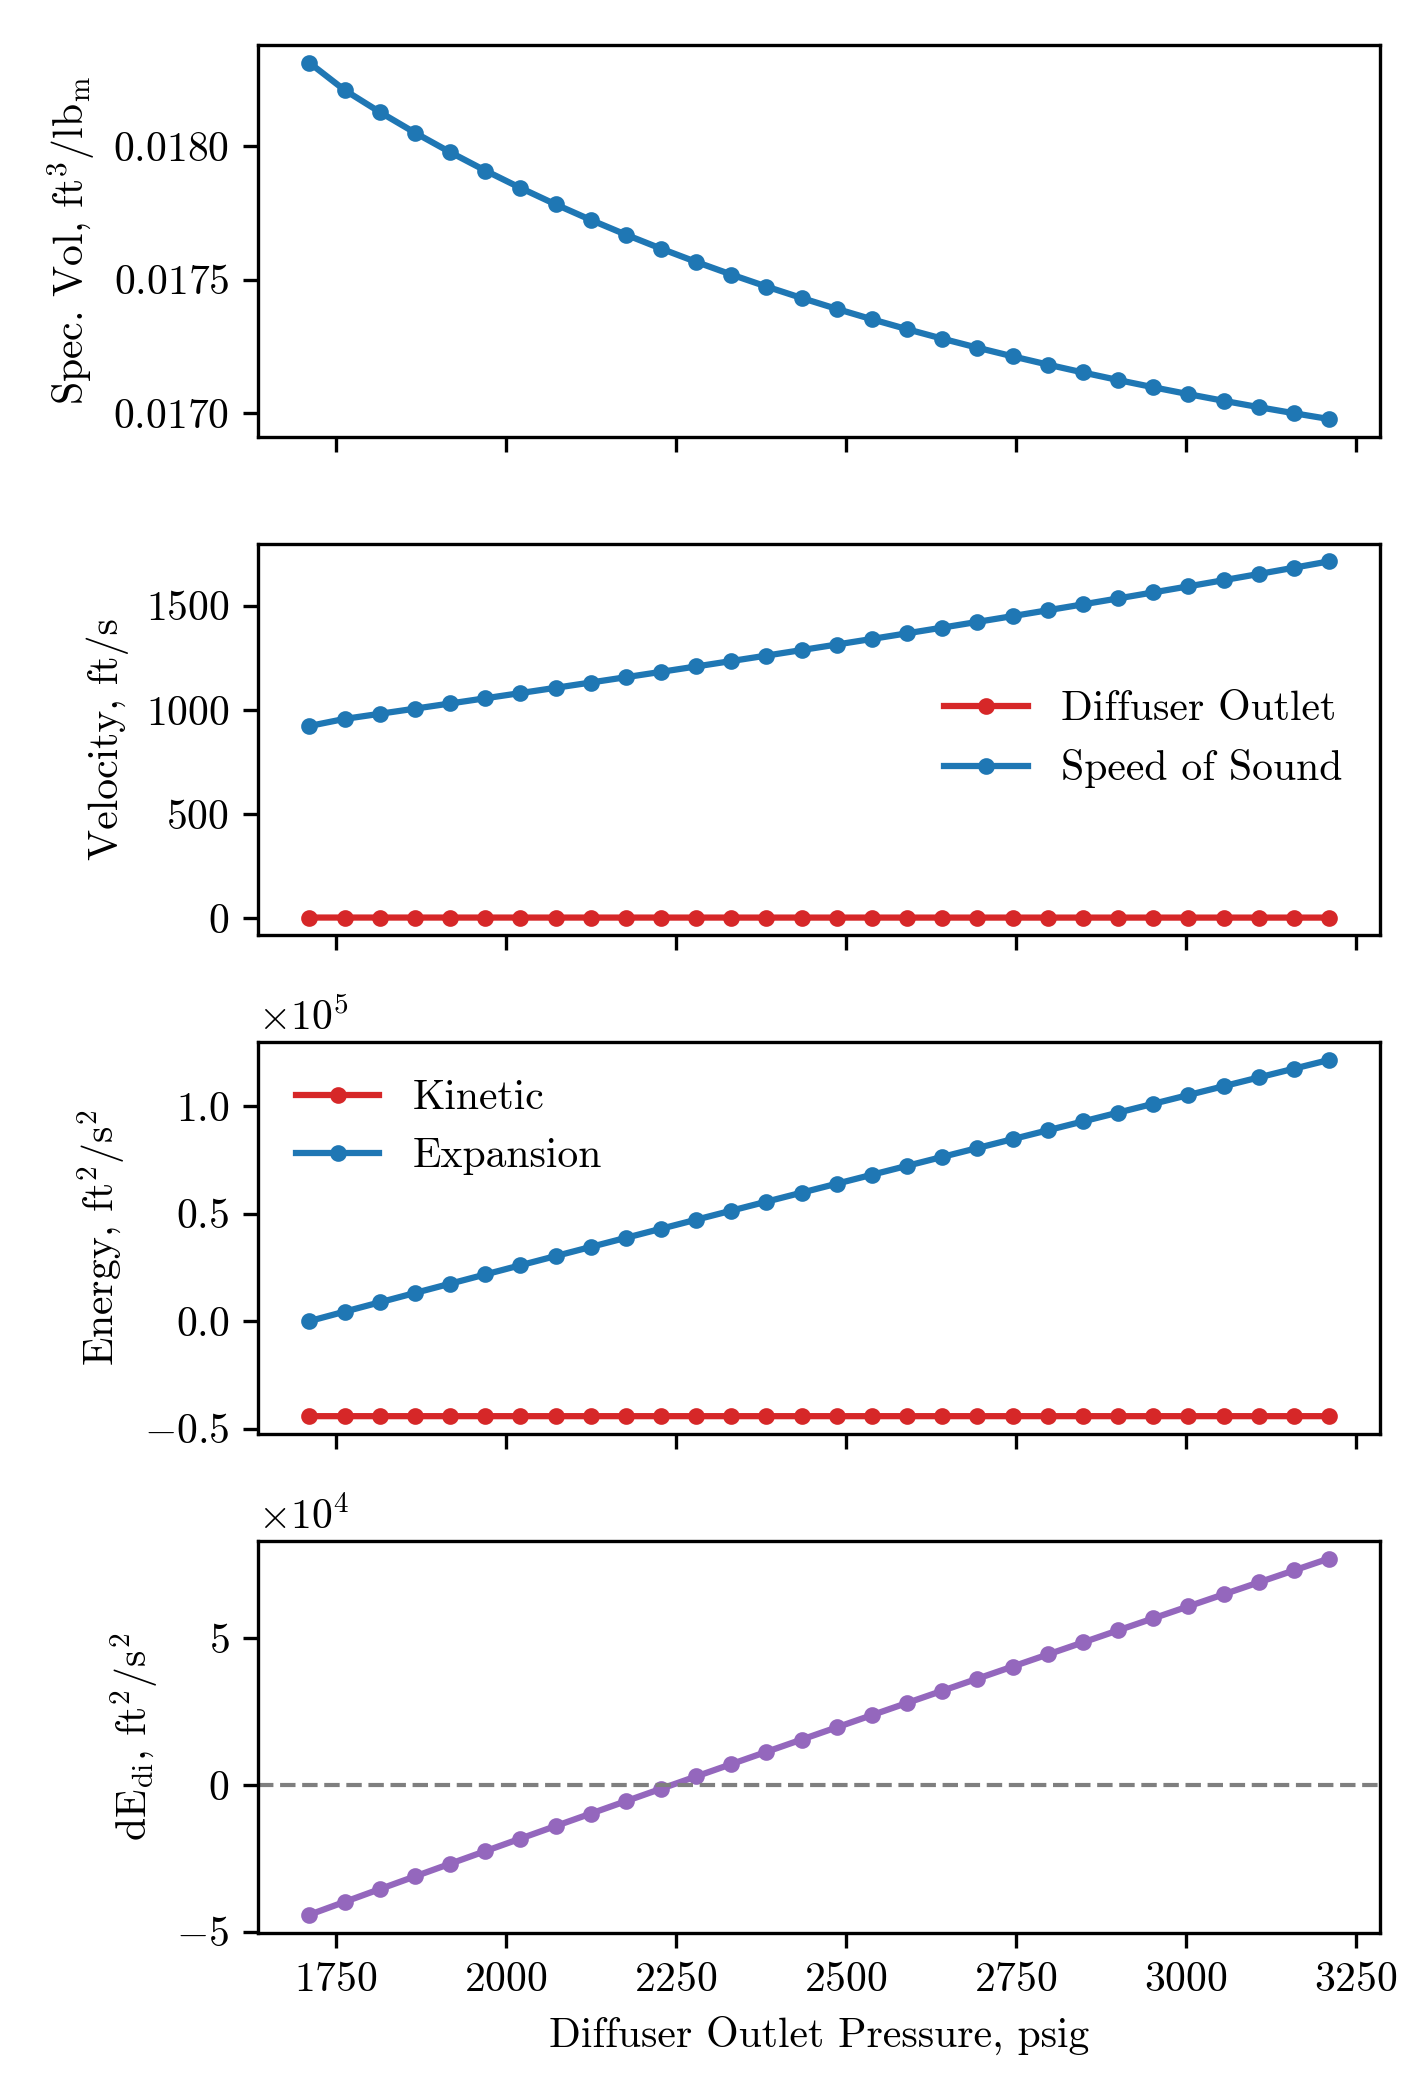
\includegraphics[scale=1]{figures/diffuser_four.png}
    \caption{Properties for Calculating Diffuser Pressure}
    \label{fig:diff_four}
\end{figure}

Figure \ref{fig:diff_four} is a plot of the the various properties required to calculate the diffuser discharge pressure. The plot and it creation are nearly identical to the throat entry. The first difference is that the starting point is on the left, at a low pressure, which builds up as kinetic energy is converted to pressure energy. The second difference is the sonic velocity is significantly far away  from the diffuser outlet velocity. This shift is due to the large influx of water that was imparted into the mixture by the nozzle.  Since the diffuser is not operating close to sonic velocity limitations, the performance of \dedi against pressure is perfectly linear.

Once the diffuser discharge pressure is found, a theoretically viable solution for all the jet pump sections has been achieved.

\section{Frictional Values}

Jet pump friction coefficients used in the model have a significant impact on the results obtained. Despite the significant impact, no prescriptive method exists for picking the coefficients. Instead a survey of literature was used. Sanger used values shown in table \ref{tab:fric_coeff_sanger} for his study on non-cavitating LJL pumps \cite{sanger_non_cav}.

\begin{table}[h]
\centering
\begin{tabular}{|c|c|c|}
\hline
Description & Symbol & Value \\
\hline
Throat Entrance & $K_{te}$ & 0.03 \\
Nozzle & $K_{nz}$ & 0.01 \\
Throat & $K_{th}$ & 0.1 \\
Diffuser & $K_{di}$ & 0.1 \\
\hline
\end{tabular}
\caption{Sanger Friction Coefficients}
\label{tab:fric_coeff_sanger}
\end{table}

The jet pumps that Sanger analyzes are referred to as low friction, based on the large throat diameters. Cunningham states that for LJG pumps with a throat diameter of less than 1/2 an inch in Table \ref{tab:fric_coeff_cunn} should be used \cite{cunn_two}.

\begin{table}[h]
\centering
\begin{tabular}{|c|c|c|}
\hline
Description & Symbol & Value \\
\hline
Throat Entrance & $K_{te}$ & 0 \\
Nozzle & $K_{nz}$ & 0 \\
Throat & $K_{th}$ & 0.41 \\
Diffuser & $K_{di}$ & 0.35 \\
\hline
\end{tabular}
\caption{Cunningham Friction Coefficients}
\label{tab:fric_coeff_cunn}
\end{table}

The Sanger and Cunningham values were taken as two extremes, a LJL and a LJG pump. In this model, an aggregate of the two frictional values are used. The friction values used in the report are shown in Table \ref{tab:fric_coeff_model}.

\begin{table}[h]
\centering
\begin{tabular}{|c|c|c|}
\hline
Description & Symbol & Value \\
\hline
Throat Entrance & $K_{te}$ & 0.03 \\
Nozzle & $K_{nz}$ & 0.01 \\
Throat & $K_{th}$ & 0.3 \\
Diffuser & $K_{di}$ & 0.3 \\
\hline
\end{tabular}
\caption{Model Friction Coefficients}
\label{tab:fric_coeff_model}
\end{table}

The frictional values in Table \ref{tab:fric_coeff_model} provided good matches on actual performance data of operating multiphase jet pumps. Only suction and discharge pressure gauges exist on the deployed jet pumps, so absolute confidence in which component is causing the pressure loss is difficult.

\section{Assembly}
To this point in the report the jet pump has be viewed in a relatively isolated manner. Some interaction with the reservoir rock and flow of power fluid in the annulus has been discussed, but nothing on the requirements for pumping the fluid to surface. The jet pump is thousands of feet below the ground and needs to generate enough head to pump the fluid to surface. To verify the capabilities, the static and frictional pressure loss in the tubing need to be accounted for.

The discharge pressure of the pump, aka the diffuser pressure, will be segregated into two separate variables. The first variable is the available discharge pressure, \pdiA. The \pdiA is the pressure the jet pump can output for a given suction pressure and power fluid conditions and was solved for in section \ref{diff_section}. The second variable is the required discharge pressure, \pdiR. The \pdiR is the pressure needed to get the fluid column from under the ground to surface. Both the static fluid column and frictional loss in the tubing need to be accounted for. The discharge pressure required takes the form of equation \eqref{pdi_req}.

\begin{equation}
P_{di}^R = P_{wh} + P_{fric} + P_{static}
\label{pdi_req}
\end{equation}

The variables are the well head pressure, frictional pressure loss in tubing and static pressure loss. Though the majority of the fluid in the tubing is water, free gas still exists and multiphase correlations need to be used. Beggs and Brill \cite{payne_multiphase} is used to calculate the liquid holdup in the pipe and friction coefficient. A term called the discharge residual is created to compare the available and required discharge pressure. 

\begin{equation}
R_{di} = P_{di}^A - P_{di}^R
\label{res_disch}
\end{equation}

For a given jet pump operating at a specific well head and power fluid pressure, the residual is only dependent on the pumps suction pressure. The suction pressure is bounded by two extremes, the minimum and maximum. The minimum suction pressure is the point where the throat entrance is operating in choked flow. The maximum suction pressure uses a ten psi draw down across the reservoir. Finding the residual for the minimum suction pressure is detailed below.

\begin{enumerate}
    \item Calculate the \textbf{minimum} suction pressure for given jet pump and IPR
    \begin{enumerate}
        \item Choked throat entrance, \dete is zero and the Mach number is one
    \end{enumerate}
    \item Solve the nozzle, throat and diffuser equations for \pdiA
    \item Solve the outflow equations for required discharge pressure \pdiR
    \begin{enumerate}
        \item Start at the wellhead pressure and solve down to the jet pump
    \end{enumerate}
    \item Calculate the discharge residual, $R_{di}$
    \begin{enumerate}
        \item If the residual is greater than or equal to zero
        \begin{enumerate}
            \item Solution is been found, well is operating in choked flow
        \end{enumerate}
        \item If the residual is less than zero
        \begin{enumerate}
            \item Find the residual of the maximum suction pressure.
        \end{enumerate}
    \end{enumerate}
\end{enumerate}

Finding the residual of the maximum suction pressure is detailed below.

\begin{enumerate}
    \item Calculate the \textbf{maximum} suction pressure for a given jet pump and IPR
    \begin{enumerate}
        \item Reservoir pressure minus 10 psi
    \end{enumerate}
    \item Solve throat entrance, nozzle, throat and diffuser equations for \pdiA
    \item Solve the outflow equations for required discharge pressure \pdiR
    \item Calculate discharge residual, $R_{di}$
    \begin{enumerate}
        \item If the residual is above zero
        \begin{enumerate}
            \item A solution exists between the minimum and maximum suction pressure
            \item The residuals of the min and max suction pressure are used as starting points for the secant method
            \item The secant method will iterate on suction pressure until residual equals zero
        \end{enumerate}
        \item If the residual is below zero
        \begin{enumerate}
            \item Well cannot lift reservoir fluid, no solution, exit function
        \end{enumerate}
    \end{enumerate}
\end{enumerate}

The secant method when iterating to find the zero discharge residual takes the form.

\begin{equation*}
    P_{su}^{k+1} = P_{su}^{k} - \frac{R_{di}^{k}(P_{su}^{k-1} - P_{su}^{k})}{R_{di}^{k-1}-R_{di}^{k}} 
\end{equation*}

The variable $k$ corresponds to iteration on the suction pressure. The starting arrays that are fed into the secant method appear as follows.

\begin{equation*}
    P_{su} = 
    \left[
    \begin{array}{c}
    P_{su}^{min} \\[6pt] 	
    P_{su}^{max} \\
    \end{array} 
    \right]
    \text{ and }
    R_{di} = 
    \left[
    \begin{array}{c}
    R_{di}(P_{su}^{min}) \\[6pt] 	
    R_{di}(P_{su}^{max}) \\
    \end{array} 
    \right]
\end{equation*}

\begin{figure}
    \centering
    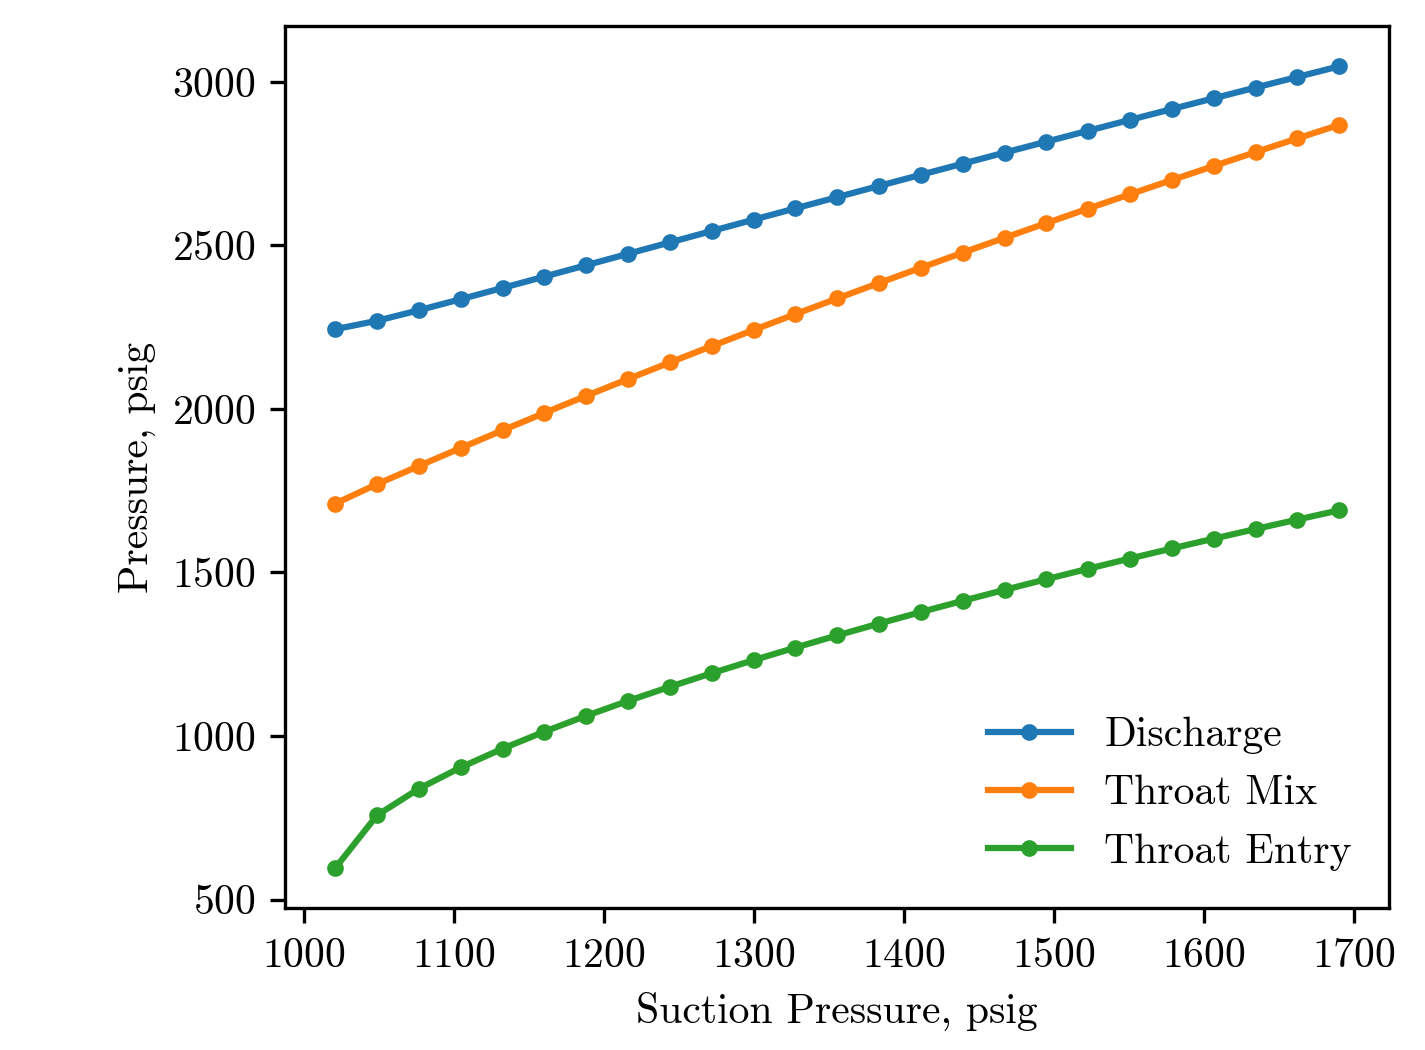
\includegraphics[scale=1]{figures/prs_relation.png}
    \caption{Pressure Relation from Varying Suction Pressure}
    \label{fig:prs_relation}
\end{figure}

Figure \ref{fig:prs_relation} shows the relationship of the suction pressure of the jet pump and the discharge. Despite the fact that the throat entry pressure is not linear to suction, the discharge is quite linear. The secant method takes advantage of this relationship to quickly iterate to a solution that drives the discharge residual to zero. Now that a jet pump model has been completed, it can be deployed to quickly understand the performance of different jet pumps in a well.

\section{Multiple Pump Runs}

Assessing a single jet pump doesn't provide much context to help with optimization of the power fluid for a well. The power fluid pressure for each well can be reduced with an individual surface choke, which would reduce the power fluid rate. The problem with choking the pressure is that it wastes valuable energy required to boost the pressure up. A better approach is to replace the subsurface jet pump to meet the required operating conditions. Controlling the flow with the jet pump nozzle tip ensures that the max pressure and in turn energy, is delivered to each well.

A batch run method is used on each oil well to run an array of multiple jet pumps. If desired, every nozzle and throat combination shown in table \ref{tab:fric_coeff_model} could be ran, but this is viewed as excessive. On the North Slope of Alaska, the largest and smallest jet pump sizes are 14C and 8B respectively. For the batch run the nozzle sizes are seven to sixteen and the throat ratios are X, A, B, C, D and E. This ensures all potential combinations are covered and provides edge cases. 

\section{Optimization Introduction}

Assessing a single jet pump doesn't provide much context to help with optimization of the power fluid for a well. The power fluid pressure for each well can be reduced with an individual surface choke, which would reduce the power fluid rate. The problem with choking the pressure is that it wastes valuable energy required to boost the pressure up. A better approach is to replace the subsurface jet pump to meet the required operating conditions. Controlling the flow with the jet pump nozzle tip ensures that the max pressure and in turn energy, is delivered to each well.

A batch run method is used on each oil well to run an array of multiple jet pumps. If desired, every nozzle and throat combination shown in table \ref{tab:fric_coeff_model} could be ran, but this is viewed as excessive. On the North Slope of Alaska, the largest and smallest jet pump sizes are 14C and 8B respectively. For the batch run the nozzle sizes are seven to sixteen and the throat ratios are X, A, B, C, D and E. This ensures all potential combinations are covered and provides edge cases.


\section{Additions}
Appendix showing derivations of the throat entrance, nozzle, diffuser and throat. Appendix discussing what PVT properties were assigned / used. Add that you don't need to worry about mach velocity limitations once past the throat entrance. \cite{kermit}

\printbibliography

\end{document}